% Chapter Template

\chapter{Theorie} % Main chapter title

\label{Chapter4} % Change X to a consecutive number; for referencing this chapter elsewhere, use \ref{ChapterX}

\lhead{Chapter 4. \emph{Material und Methoden}} % Change X to a consecutive number; this is for the header on each page - perhaps a shortened title

%-----------------------------------
%	THEORIE
%-----------------------------------

\section{Grundlagen und Definitionen}
In diesem Kapitel werden wichtige Begriffe vorgestellt, die im Verlauf der weiteren Arbeit von Bedeutung sind.

%-----------------------------------
%	WORKFLOW CASES
%-----------------------------------
\subsection{Prozess Schemata und Instanzen}

Ein Prozessschema \textbf{W = $\{T,D\}$} mit n $\in \mathbb{N}$ ist eine Menge von Aktivitäten \textbf{T = $\{t_1,t_2,...,t_n\}$} und einer Menge \textbf{D} von Abhängigkeiten, welche bestimmen, in welcher Reihenfolge die einzelnen Aktivitäten ausgeführt werden bzw von welchen Parametern abhängt, ob sie ausgeführt werden müssen, oder nicht. Die Menge der Aktivitäten muss mindestens eine Startaktivität haben, kann aber mehrere terminierende Aktivitäten beinhalten, die gleichberechtigt den Prozess abschließen.
$t_{ij}$ bezeichnet hierbei die Aktivität $t_j$ aus dem Prozessschema $W_i$. \\

\begin{figure}[ht]
	\centering
  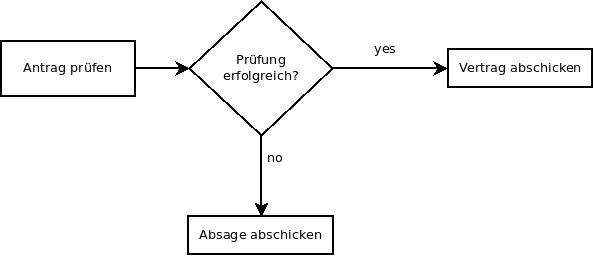
\includegraphics[width=0.7\textwidth]{Figures/sampleW}
	\caption{einfaches Beispiel eines Prozessschemas}
Ein einfaches Beispiel für das Schema eines Prozesses mit einem Start und zwei finalen Aktivitäten.In Abhängigkeit davon, welcher Wert für x berechnet wird, wird der Prozess entweder sofort abgebrochen, oder es werden weitere Aktivitäten ausgeführt.
	\label{fig2}
\end{figure}

Ein Prozessschema kann mehrere Instanzen besitzen, die mit \textbf{W$_i^k$} gekennzeichnet werden.
Eine Prozessinstanz $W_i^k$ ist eine Menge von Instanzen $T_i^k$ der zugehörigen Aktivitäten. Dabei ist $|T_i| \subseteq |T|$ eine Teilmenge aller möglichen Aktivitäten des zugehörigen Schemas, da einzelne Aktivitäten unter Umständen aufgrund der Abhängigkeiten nicht ausgeführt werden müssen.


%-----------------------------------
%	ACTIVITIES TASKS
%-----------------------------------
\subsection{Aktivitäten}
Eine Aktivität ist ein atomares Event, dh. eine in sich abgeschlossene Aufgabe im Kontext eines Prozesses. Sie haben eine definierte Menge von potentiellen Rollen und Nutzern, die die Erlaubnis besitzen, diese Aufgabe auszuführen. Sobald sie einem Nutzer zugewiesen wurde, kann niemand anderes mehr die Aufgabe annehmen. Das bedeutet, dass jede Aktivität einen eindeutigen Nutzer und eine eindeutige Rolle hat, welcher sie ausgeführt hat.

Des weiteren besitzen die Aktivitäten einen eindeutigen Zeitstempel $\tau$, zu dessen Zeitpunkt sie ausgeführt wurden. Diese Zeitstempel bestimmen eine Ordnung $<T, \leq>$. Es gilt nämlich $t_1 < t_2 $, wenn $t_1$ vor $t_2$ ausgeführt wurde, dh. timestamp($t_1$) $<$ timestamp($t_2$).


Sie besitzen 3 verschiedene Zustände: Assigned, Started und Completed welche durch Activities/Events in den nächsten Zustand übergeleitet werden. Das MXML Modell unterstützt 13 verschiedene Events, die sich in ihrer Bennenung bei den einzelnen Programmen unterscheiden können. Events können auch feiner gegliedert sein, bzw es kann auch sein, dass nur eine Teilmenge davon verwendet wird. In dieser Arbeit gehen wir davon aus, dass es folgende Events gibt: started, assigned, completed, ...




\begin{figure}[ht]
	\centering
  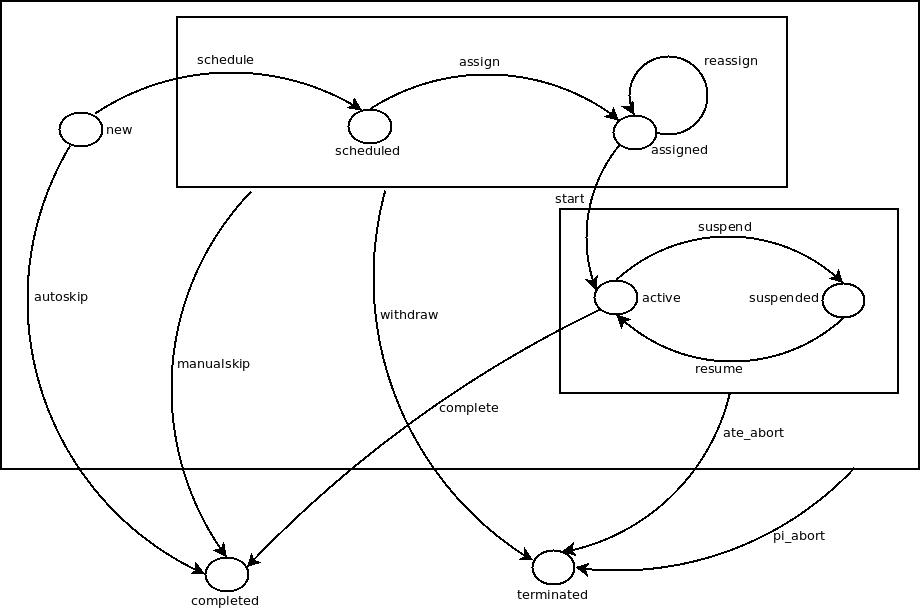
\includegraphics[width=0.9\textwidth]{Figures/Taskevents}
	\caption{Tasks und Events}
	\label{fig2}
\end{figure}
 

%-----------------------------------
%	ROLLENMODELL
%-----------------------------------
\subsection{Rollenmodell und Authorisierung}
Sei T = $\{t_1,t_2,...t_m\}$, $m\in\mathbb{N}$ eine Menge von Tasks, R = $\{r_1,r_2,...t_n\}$, $n\in\mathbb{N}$ eine Menge von Rollen, und U = $\{u_1,u_2,...u_l\}$,$l\in\mathbb{N}$ eine Menge von Usern.

\begin{figure}[ht]
	\centering
  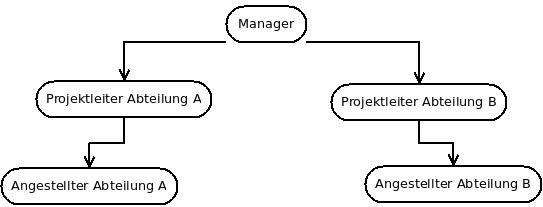
\includegraphics[width=0.9\textwidth]{Figures/Rollenmodell}
	\caption{Beispiel Rollenmodell}
	\label{fig:examplerolemodel}
\end{figure}

Eine \textbf{Authorisierung} ist eine Menge von potentiellen Nutzer und Rollen, denen es erlaubt ist, einen Task auszuführen. Eine Authorisierung besteht aus den Tupeln $$\textbf{TR} = (T\times R)$$ und $$\textbf{UR} = (U\times R)$$, welche eine n:m-Beziehung zwischen Tasks und Rollen, bzw zwischen Usern und Rollen kennzeichnen. Das bedeutet, dass User mit Rollen in der User-Rollen Beziehung assoziiert werden und Tasks mit Rollen in der Tast-Rollen Beziehung assoziiert werden.\\
Sei nun $$\textbf{R(t)} = \{r_m \in R: \exists(t_k, r_m) \in TR(t)\}$$
$$\textbf{U(t)} = \{u_n \in U: \exists(u_n, r_m) \in UR, r_m \in R(t)\}$$
Mit anderen Worten ist R(t) die Menge aller Rollen, die authorisiert sind, einen Task auszuführen und U(t) die Menge alles User, die authorisiert sind, einem Task zugeteilt zu werden.\\
Eine \textbf{Zuweisung} ist die konkrete Ausführung eines Tasks durch einen User.

Ein \textbf{hierarchisches Rollenmodell} ist eine geordnete Menge von Beziehungen zwischen Rollen $<R, \leq>$. Wenn $r_1, r_2 \in R$ und $r_1 < r_2$, dann dominiert die Rolle $r_2$ die Rolle $r_1$ in Bezug auf die organisatorische Rollenhierarchie. In Abb. \ref{fig:examplerolemodel} dominiert die Rolle "Projektleiter" die Rolle "Angestellter", das bedeutet, dass der "Projektleiter" alle Tasks ausführen darf, die der Rolle "Angestellter" zugeordnet wurde.
Die Rolle und all ihre Elternrollen bis zur Wurzel können einem Task zugewiesen werden.

\cite{wolter_modeling_of_TBAC_in_BPMN}

%-----------------------------------
%	ZEITMODELL
%-----------------------------------
\subsection{Zeitmodell}
Das Zeitmodell ist ein Tupel T = ($\Tau;\leq$).\\
$\Tau$ ist eine Menge von \textit{Zeitpunkten} $\tau$ und $\leq$ eine total Ordnung auf $\Tau$.
Ein \textit{Zeitinterval}$[\tau_a, \tau_b]$ ist eine Menge von Zeitpunkten $\tau \in \Tau$ mit $\tau_a \leq \tau \leq \tau_b$.
Ein Zeitinterval $[\tau_a, \tau_b]$ wird als leer bezeichnet, falss $\tau_b \leq \tau_a$.


TODO darauf achten, dass hier Konsistenz herrscht mit ts, tp, ... in der späteren Grammatikdefinition.
\cite{warner_inter_instance}

%-----------------------------------
%	Event Logs
%-----------------------------------
\subsection{Event Logs}

EventLogs sind Abbildungen von Workflows. Ein EventLog kann durchaus unvollständig sein bzw Fehler beinhalten. Jedoch wird in dieser Arbeit von einer "Closed World" davon ausgegangen.


\begin{figure}[ht]
	\centering
  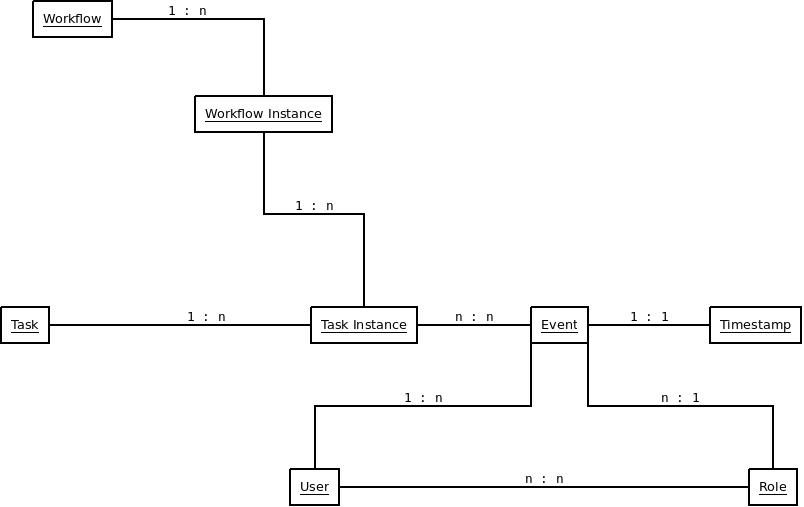
\includegraphics[width=0.9\textwidth]{Figures/WorkflowOntology}
	\caption{Ontologie eines Workflows}
	\label{fig:ontology}
\end{figure}


\begin{table}[h]
  \centering
  \begin{tabular}{|c|c|c|c|c|c|}
  \hline
  caseID & Task & User & Role & Timestamp & EventType\\
  \hline
  0 & Approach check &'Mark' &'Admin' &1999-12-13T12:22:15 & start\\
  0 & Pay check & 'Theo' &'Azubi' &1999-12-13T12:22:16 & start\\
  1 & Approach check &'Lucy' & 'Azubi' &1999-12-13T12:22:17 &start\\
  1 & Pay check &'Mark' & 'Admin' &1999-12-13T12:22:18 & abort\\
  0 & Revoke check & 'Theo' & 'Clerk' & 1999-12-13T12:22:19 & start\\
  \hline
  \end{tabular}
\\
Das ist nur ein Auszug und kein vollständiger Log. Es können auch weitere Daten vorhanden sein, die hier nicht dargestellt werden.
  \caption{Beispiel Log Einträge. }
  \label{tab:examplelog}
\end{table}


%-----------------------------------
%	Definition Constraints
%-----------------------------------
\subsection{Definition Constraints}
Constraints sind Regeln bzw Einschränkungen, die aus dem Verlauf von vorhergehenden Tasks resultieren.

%-----------------------------------
%	Security policy
%-----------------------------------
\subsection{Schutzziele}
\textbf{Autorisierung}\\
Welche Subjekte bzw Rollen dürfen auf welche Ressourcen zugreifen? Da es in größeren Unternehmen komplex werden kann, wurde das Rollenmodell zur Vereinfachung entwickelt\\
\textbf{Nutzungskontrolle}\\
Regelt die Art der Nutzung. RWX, begrenzte Anzahl an Zugriffen, bzw Verpflichutung einer Löschoperation (weiteren, resultierenden Handlungen) nach Zugriff(Kontrollfluss)\\
\textbf{Interessenskonflikt}\\
Unterbindung von unzulässiger Ausnutzung von insider-Wissen. Chinese Wall Modell.\\
\textbf{Funktionstrennung}\\
Bestimmte Aufgaben dürfen nicht vom selben Subjekt, Rolle, Abteilung, ausgeführt werden. Unterbindung von kriminellen Handlungen und Betrug.\\
\textbf{Aufgabenbindung}\\
Gegenteil von Funktionstrennung\\
\textbf{Mehr-Augen-Kontrolle}\\
kritische Aktivität im Prozess darf nicht von einer einzelnen Person ausgeführt werden. Das wäre bei mir Cardinality Constraints, wenn eine Aktivität aus mehreren Tasks besteht.\\
\textbf{Isolation}\\
keine Datenlecks innerhalb eines Prozesses bzw zwischen mehreren Prozessen.\\





\cite{mueller_accorsi}
\section{Herleitung Constraints}



\subsection{Ein praktisches Beispiel mit vielen Einschränkungen}
Das folgende Beispiel wurde in leicht veränderter Form \cite{wolter_modeling_of_TBAC_in_BPMN} entnommen.
 Blabla Erklärung des Workflows
\begin{figure}[ht]
	\centering
  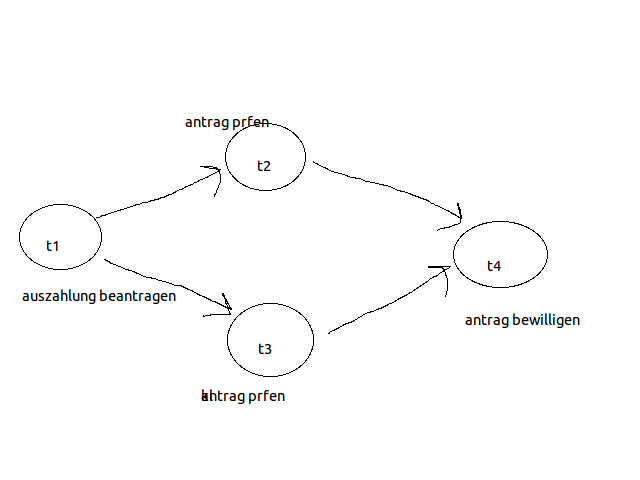
\includegraphics[width=0.9\textwidth]{Figures/Workflow}
	\caption{Workflow}
	\label{fig:Workflow}
\end{figure}
 Folgende Einschränkungen und Regeln sind gewünscht:\\

\begin{enumerate}
\item (Der Kontakt mit Kunden) T1 und T6 muss vom Kundenberater erledigt werden
\item Um den Kunden nicht zu lange warten zu lassen, sollte der Kunde spätestens 3 Tage nach erstem Kontakt über das Ergebnis informiert werden (timestamp(T6) $<$ timestamp(T1) + 3D)
\item Um zu verhindern, dass Fehler durch Überlastung passieren, darf jeder Mitarbeiter am Tag höchstens 100 Tasks beartbeiten.
\item Den Antrag annehmen (T1) und den Antrag prüfen(T2, T3) sollten von verschiedenen Personen erledigt werden (4 Augen Prinzip).
\item Ferner sollten auch die zwei Prüfungen von verschiedenen Mitarbeitern vollzogen werden. T3 muss durch den Bank Manager erfolgen.
\item Wenn ein Mitarbeiter 5x einem Task zugewiesen wird und ihn dann abbricht, darf er nicht mehr an dem Task arbeiten.
\item Es dürfen keine Anträge von Verwandten geprüft werden.
\item Es dürfen auch höchstens 3 mal Mitarbeiter an den Anträgen des jeweils anderen Verwandten arbeiten.
\item Ein Mitarbeiter darf bei dem selben Kunden höchstens Kredite bis 100000 Euro prüfen.
\item Es dürfen hochstens 3 mal die selben Personen an T2 und T3 arbeiten
\end{enumerate}


%
% Arten von Constraints
%
\subsection{Arten von Constraints - Herleitung}

Generell kann man verschiedene Arten von Regeln erkennen.\\

\begin{figure}[ht]
	\centering
  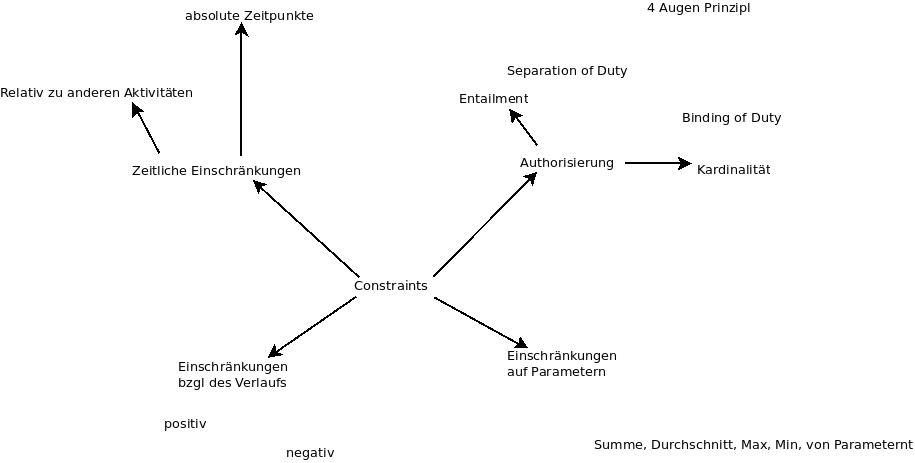
\includegraphics[width=0.9\textwidth]{Figures/Constraints}
	\caption{Typen von Einschränkungen und regeln}
	\label{fig:constraints}
\end{figure}

\subsubsection{sich gegenseitig ausschließende Tasks (Conflicting Tasks)}
TODO: kommt das zur Constraint Sammlung?
In manchen Fällen kann man Tasks nicht verschiedenen Rollen zuweisen  ohne die exisitierenden Rollen derart zu segmentieren, dass die schwer zu verwalten sind in Bezug auf das organsiatorische Modell. Außerdem können Rollenhierarchien dazu verwendet werden, in zwei verschiedenen Rollen zu agieren, die eigentlich getrennt waren. ZB könnte ein Manager als ein Clerk und gleichzeitig als sein eigenener Supervisor handeln.\\
Deswegen definieren wir \textbf{TC} $\subset$ T als eine Menge von \textbf{kollidierenden Tasks}. TC beinhaltet Tasks, deren Allokation von der Allokation von vorhergehend ausgeführten Tasks aus TC abhängt. Diese Abhängigkeit wird als Abhängigkeit zwischen Tasks aus TC beschrieben. $t_c\in TC$ gilt als entailed Task von $t_m\in TC$, wenn die Allokation von $t_n$ von der Allokation von $t_m$ eingeschränkt wird, mit $t_m<t_n$.
\cite{wolter_modeling_of_TBAC_in_BPMN}

\subsubsection{Entailment Constraint}
c=(TC, $n_u$,$m_{th}$) mit $n_u$ als minimale Anzahl an verschiedenen Usern, die einem Task zugewiesen werden müssen. Wenn $t_{ki}$ eine Instanz des Tasks $t_k$ ist, dann ist $m_th$ der Grenzwert von der Summe der Task Instanzen, denen ein User zugewiesen sein darf.
\cite{wolter_modeling_of_TBAC_in_BPMN}

zeitliche Beschränkungen
--absolute Einschränkungen\\
--relative Einschränkungen\\
Akkumulationen\\
Separation of Duty\\
Binding of Duty Constraints\\
Cardinality Constraints\\
Workflow Soundness\\
--Bild dazu\\

\subsection{Gültigkeitsbereich von Constraints}

\textbf{Intra-Instanz}\\
Die meisten Ansätze beziehen sich auf Regeln, die in Bezug zu einer Prozessinstanz stehen. Hier gilt, dass die Prozessinstanz für alle Aktivitäten die selbe ist.
\textbf{Inter Instanz}\\
Geht man davon aus, dass gleiche Arbeitsabläufe zum selben Prozessschema gehören, dann ist dieser konstant. Die Aktivitäten können jedoch zu verschiedenen Prozessinstanzen gehören.
\textbf{Inter-Prozess}\\
Die Regeln beziehen sich auf alle Aktivitäten, unabhängig davon, zu welcher Prozessinstanz oder welchem Prozessschema sie gehören.

%
% Vorüberlegungen zur Grammatik
%
\section{Vorüberlegungen zur Grammatik}
\subsection{Was muss sie können?}
- Sie sollte Regeln auf Basis der verschiedenen Aktivitäten aufstellen können\\
- Rollenmodell berücksichtigen, dh Möglichkeit, es anzugeben\\
- Ziel ist eine möglichst intuitive Notation\\
- arithmetische Operationen auf Grundbiveau sollten möglich sein, um Bedingungen in Bezug auf Zeiten und andere numerische Werte  aufstellen zu können.
\subsection{Weiterführende Fragen}
-Woran erkennt man den Kontext der Constraints? \\
-Welches Rollenmodell wird benutzt, und welche Auswirkungen hat es auf die Grammatik?\\
-Was passiert bei fehlenden Einträgen, oder falschen Einträgen?\\
-Soll Negation erlaubt sein?\\
-Was definiert der Timestamp, wenn es sich doch nur auf verschiedene Events bezieht?\\
-Soll auf der Event Basis oder auf der Task Basis gearbeitet werden?

%
% Definition der Grammatik
%
\section{Definition der Grammatik}
\subsection{Basis von Werten, Aussagen...}
Zuerst Herleitung, was wir genau an Aussagen brauchen\\
\subsubsection{Argumenttypen - Variablen und Konstanten}

Man kann einem Prädikat entweder eine Variable oder eine Konstante des jeweiligen Typs übergeben. Variablen müssen mit einem Großbuchstaben beginnen und können die Zeichen [A-Z][a-z][0-9] enthalten. Konstanten können aus beliebigen Zeichen bestehen, müssen aber innerhlab zwei einfacher Anführungsstriche stehen. Die Grammatik ist dynamisch typisiert, das heißt der jeweilige Typ wird aus dem Kontext bestimmt.

\begin{enumerate}
\item Originator: UT = UV + UC, mit UV Variablen ueber Originator, UC Konstanten
\item Rollen: RT = RV + RC
\item zeitliche Parameter
\item Eventtypen: ET = EV + EC, mit EC $\in\{started, completed,...\}$
\end{enumerate}

\subsubsection{Prädikate}
Prädikate sind Aussagen über bestimmte Zustände. Es gibt verschiedene Typen. Externe Informationen, Spezifikation, Status, Enforcement und Konditionell. \\

Externe Informationen (Tabelle \ref{tab:extern}) sind Aussagen, die nicht direkt mit der Workflow Spezifikation zu tun haben aber dennoch relevant für den Ablauf sein könnten. Diese Prädikate müssen explizit in den Regeln gesetzt werden, da es sonst zu keinem Ergebnis führt.
\begin{table}[h]
\begin{tabular} {|p{6cm}|p{10cm}|}
\hline
\textbf{Prädikat} & \textbf{Beschreibung}\\
\hline
UT is related to UT 		& Beide User sind verwandt \\
\hline
UT is partner fo UT		& Beide Akteure sind Partner \\
\hline
UT is in same group as UT	& Beide Akteure sind in der selben Gruppe, Abteilung\\
\hline
\end{tabular}
\caption{Prädikate für externe Informationen. Das sind nur drei Vorlagen. Dem Programmierer ist selbst überlassen, wie er diese Prädikate interpretieren will.}
\label{tab:extern}
\end{table}

Spezifikationsprädikate (Tabelle \ref{tab:specification}) bestimmen die Beziehungen und Zugehörigkeit zwischen Nutzern, Rollen und Tasks. Sie Sollten genauso gesetzt werden, wie die Spezifikation war, als der Workflow ausgeführt wurde.
\begin{table}[h]
\begin{tabular} {|p{6cm}|p{10cm}|}
\hline
\textbf{Prädikat} & \textbf{Beschreibung}\\
\hline
'role' RT 'can execute' TT	& RT ist in  R(TT)\\
\hline
'user' UT 'can execute' TT 	& UT ist in U(TT)\\
\hline
'user' UT 'belongs to role' RT  & (UT,RT) ist in UR\\
\hline
RT 'is glb of' TT 		& greatest lower bound. TT muss mindestens mit Rolle RT ausgeführt werden\tnote{1}\\
\hline
RT 'is lub' TT 			& lowest upper bound. TT darf höchstens mit Rolle RT ausgeführt werden\tnote{1}\\
\hline
RT 'dominates' RT 		& Rolle 1 dominiert Rolle 2\tnote{1}\\
\hline
'critical{\_}task{\_}pair(' TT ',' TT ')'& Die beiden Tasks sind ein kritisches Paar. Die User werden markiert, die dieses Paar ausführen\\
\hline
\end{tabular}
\begin{tablenotes}\footnotesize 
\item[1] In Bezug auf die jeweilige Rollenhierarchie 
\end{tablenotes}
\caption{Prädikate für die Spezifikation von ...}
\label{tab:specification}
\end{table}

Statusprädikate (Tabelle \ref{tab:status}) sind Aussagen über Aktivitäten. Diese werden später mit den Informationen aus den Logs verglichen. 
\begin{table}[h]
\begin{tabular} {|p{6cm}|p{10cm}|}
\hline
\textbf{Prädikat} & \textbf{Beschreibung}\\
\hline
('user')? UT 'executed' TT      & Ut hat TT so ausgeführt, dass TT completed ??\\
\hline
'role' RT 'executed' TT		& RT hat TT ausgeführt\\
\hline
UT 'is assigned to' TT		& UT wurde TT zugewiesen\\
\hline
TT 'aborted'			& TT ist abgebrochen\\
\hline
TT 'succeeded'			& TT hat geklappt \\
\hline
UT 'is collaborator of' UT	& UT sind alle Akteure, die an criticalTaskPair gearbeitet haben\\
\hline
\end{tabular}
\caption{Prädikate, um Aussgen über den Status in die Regeln mit einbeziehen zu können}
\label{tab:status}
\end{table}

Konditionelle Prädikate (Tabelle \ref{tab:conditional})
\begin{table}[h]
\begin{tabular} {|p{6cm}|p{10cm}|}
\hline
\textbf{Prädikat} & \textbf{Beschreibung}\\
\hline
number where body is RES		& Zählt die Anzahl der verschiedenen Lösungen für body \\
\hline
number of VAR where body is RES	& Zählt die Anzahl der verschiedenen Lösungen für VAR, die body erfüllen. VAR muss mindestens einmal in body vorkommen.\\
\hline
sum of NT where body is RES		& Gibt die Summe von NT zurück. NT muss im body enthalten sein und zählt alle Lösungen mit. NT muss\\
\hline
avg of NT ?TauT? where body is RES		& Gibt den Durchschnitt von NT zurück.\\
\hline
min of NT ?TauT? where body is RES		& Gibt das Minimum von NT zurück.\\
\hline
max of NT ?TauT? where body is RES		& Gibt das Maximum von NT zurück.\\
\hline
\end{tabular}
Das Resultat wird in der Variable gespeichtert, die anstelle von RES definiert wurde. Body ist eine Konjunktion von Status- , Externen und Spezifikationsprädikaten.
\caption{Prädikate für Aussagen über die Akkumulation von Werten}
\label{tab:conditional}
\end{table}


Vergleiche (Tabelle \ref{tab:comparison})
\begin{table}[h]
\begin{tabular} {|p{6cm}|p{10cm}|}
\hline
\textbf{Prädikat} & \textbf{Beschreibung}\\
\hline
 $= | !=$		& ww \\
 $< | <= | > | >=$   	& dd \\
\hline
\end{tabular}
...
\caption{Vergleiche}
\label{tab:comparison}
\end{table}

Operationen (Tabelle \ref{tab:operations})
\begin{table}[h]
\begin{tabular} {|p{6cm}|p{10cm}|}
\hline
\textbf{Prädikat} & \textbf{Beschreibung}\\
\hline
 $+ |-$		& bb \\
 $ * | / $   	& bb \\
\hline
\end{tabular}
...
\caption{Operationsn}
\label{tab:operations}
\end{table}

Kopfprädikate. Diese müssen im Kopf einer Regel stehen, und dürfen nicht im Körper vorkommen. (Tabelle \ref{tab:head})
\begin{table}[h]
\begin{tabular} {|p{6cm}|p{10cm}|}
\hline
\textbf{Prädikat} & \textbf{Beschreibung}\\
\hline
UT cannot execute TT		& ww \\
UT must execute TT  		& dd \\
RT cannot execute TT		& \\
RT must execute TT		& \\
illegal execution		& \\
\hline
\end{tabular}
...
\caption{Prädikate für den Kopf einer Regel}
\label{tab:head}
\end{table}



\subsubsection{Regeln}
Regeln (Constraints sind Schlussfolgerungen, die sich aus Vorbedingungen ergeben. Es gibt positive und negative. Die positiven sagen, dass etwas passieren muss, die negativen verbieten, dass etwas passiert)\\
Ableitung,...\\
Die Köper der Regel werden als Konjunktion (Disjunktion ist ebenfalls möglich, jedoch nicht zwingend notwendig - siehe Kapitel \ref{sec:disjunction}) von Prädikaten gebildet.\\

\begin{verbatim}
IF body THEN head
\end{verbatim}

Der Körper - body ...\\
Der Kopf der Regel - head darf nur aus 

\subsection{Grammatik - Syntax}
Für ein besseres Verständnis der Definition erst einmal ein kurzes Beispiel:\\

\begin{verbatim}
SET 'Mark Maier' is related to 'Max Mueller'
IF USER_A executed 'Kredit beantragen' AND USER_A is related to USER_B
  THEN USER_B cannot execute 'Kredit prüfen'
\end{verbatim}
\begin{figure}[!h]
\caption{Beispiel Spezifikation einer einfachen Regel}
\label{fig:demorulefile}
\end{figure}

Konstanten sind als 'String' , Variablen ohne \\
Welche Zeichen darf man wo verwenden?\\
Verfügbare Literale\\
Syntax\\
Fakten: SET extern|workflow \\
Regeln: 	IF (..|..) (AND (..|..)*) \\
THEN (..|..) \\
WHERE t.name = t2.name AND  ...\\

\subsubsection{Definition eigener Prädikate}
Es kann nötig erscheinen, eigene Prädikate zu definieren. Zum Beispiel um weitere Personengruppen anzulegen oder um Abkürzungen für Zusammenhänge zu erstellen. Dafür gibt es die Möglichkeit, ein Prädikat mittels des Schlüsselwortes "Def" zu Beginn der Regeldefinitionen zu setzen. In der Definition wird der Typ der Argumente gesetzt. Man hat die Wahl zwischen UT,RT,TT,...
Um die eigenen Prädikate nutzen zu können, muss man jedoch beachten, dass sie bei der Definition noch keinen "Wert" haben. Entweder muss man sie dann mit "SET" setzen oder mann kann ihnen eine Regel erstellen. Um die Prädikate für den Parser und die weitere Verarbeitung eindeutig sind, sind sie an eine spezielle Form gebunden: predicate{\_}name( ARGType,...).

\begin{verbatim}
DEF suspicious(UT)
DEF skipped(TT)
DEF aborted(UT,TT)

SET suspicous('Max Neuer')
SET suspicous('Tom Weisser')

IF EventType(ACTIVITY).'skipped' THEN skipped(ACTIVITY)
IF ACTOR executed ACTIVITY AND EventType(ACTIVITY).'aborted' THEN aborted(ACTOR, ACTIVITY)
\end{verbatim}
\begin{figure}[!h]
\caption{Definition eigener Prädikate. .. wurde gesetzt, .. hat eine eigene Regel}
\label{fig:define}
\end{figure}

%
% Erklärungen zur Grammatik
%
\section{Verwendung der Grammatik, Erklärungen}
Wenn sich etwas auf jede Instanz einzeln beziehen muss, muss Task1.workflow.instance = Task2.workflow.instance\\
Eignet sich für hierarchisches und auch für normales Rollenmodell. Hängt nur davon ab, ob die Hierarchie als Fakt gesetzt wurde.\\
User und ihre Rollenzuweisungen müssen nicht explizit angegeben werden. Nur wenn man das für die Vergleiche braucht.\\
Beziehung zwischen critical task pair und collaborateur.
\subsection{Disjunktion}
\label{sec:disjunction}
Es wird wenige Fälle geben, in denen eine Disjunktion von Klauseln notwendig ist. Um besser nachvollziehen zu können, zu welchem Fall eine Regelverletzung gehört, ist es oft sogar sinnvoller, eine Regel, die mehrere Fälle erlaubt, und mehrere Regeln aufzuteilen. Jedoch kann es verwendet werden, um Kardinalitätsaussagen einfacher darstelen zu können (TODO: mein Beispiel auf einem Zettel suchen), deswegen wird Disjunktion in der Grammatik erlaubt. Um die ??Assoziativität?? deutlich zumachen, müssen Disjunktionen in einer Klammer stehen. Disjunktion ohne umgebende Klammern ist nicht erlaubt. Disjunktionen von Konjunktionstermen ist nicht erlaubt.

\begin{verbatim}
IF (User executed 'task1' OR USER executed 'task2')
THEN User cannot execute 'task3'
\end{verbatim}
\begin{figure}[!h]
\caption{Disjunktion im Körper einer Regel. Man beachte, dass jede Disjunktion von umschließenden Klammern umgeben sein muss.}
\label{fig:disjunction1}
\end{figure}

Im Kopf einer Regel ist Disjunktion nicht erlaubt. Die Regel muss in zwei getrennte Regeln gespalten werden.

\begin{verbatim}
IF User executed 'task1'
THEN User cannot execute 'task2'

IF User executed 'task1'
THEN User cannot execute 'task3'
\end{verbatim}
\begin{figure}[!h]
\caption{Disjunktion im Kopfbereich ist nicht erlaubt. Es müssen zwei getrennte Regeln erstellt werden.}
\label{fig:disjunction2}
\end{figure}

\subsection{Umgang mit verschiedenen Rollenmodellen}
In den meisten Systemen wird ein hierarchisches Rollenmodell eingesetzt. Man ist bei der Analyse mit diesem Modelchecker nicht daran gebunden.

\subsection{Negation}
Negation wird ebenfalls für die Bildung der meisten Regeln nicht benötigt, wird hier aber der Vollständigkeit halber erlaubt. Dabei gilt hier das Prinzip der \textbf{negation as failure}. Da nicht garantiert werden kann, dass ein Arbeitsablauf vollständig und korrekt geloggt wurde, muss man sich hier darauf einigen, dass das "nicht-vorhandensein" einer Klausel trotzdem mit der Negation dieser Klausel gleichzusetzen ist. Sollte das ein Fehler sein, entsteht ein False-positive Eintrag, dh. es wird ein Fehler zuviel angezeigt.



%
% Nochmal konkretes Beispiel
%
\section{konkretes Beispiel}
Die zuvor gefundenen Beispiele wären mit der neuen Grammtik:\\
\begin{verbatim}
/* C1 */
IF NUMBER OF USER executed TASK IS N AND N > 5
  THEN USER cannot execute TASK
\end{verbatim}
\begin{figure}[!h]
\caption{Regeln für unsere gefundenen Beispiele}
\label{fig:resultrulefile}
\end{figure}
